\section{Технологическая часть}

В данной части будет обоснован выбор графического API, языка программирования и среды разработки, которые будут использоваться при разработке программного обеспечения.
Также будет приведена UML-диаграмма классов, описывающая структуру программы.
Будет продемонстрирован интерфейс, и будут приведены примеры работы программы.

\subsection{Средства реализации}

Далее будет обоснован выбор языка программирования и средств разработки, использованных при разработке программы.

\subsubsection{Выбор графического API}

В качестве используемого графического API был выбран OpenGL \cite{opengl} по следующим причинам:
\begin{itemize}
    \item кроссплатформенность (в отличие от DirectX \cite{dx});
    \item простота инициализации (в отличие от Vulkan \cite{vk});
    \item использование вычислительных мощностей графического ускорителя (в отличие от рендеринга на процессоре).
    % \item спецификация OpenGL реализована в драйверах большинства массовых видеокарт (NVIDIA, AMD, Intel), в связи с чем приложение возможно будет запустить практически на любом персональном компьютере.
\end{itemize}

\subsubsection{Выбор языка программирования}

В качестве используемого языка программирования был выбран C++ по следующим причинам:
\begin{itemize}
    % \item язык широко используется при разработке графических приложений;
    % \item наличие комплияторов, генерирующих высокопроизводительный исполняемый код;
    % \item язык типизирован, в связи с чем в процессе разработки возникает меньше ошибок времени выполнения;
    \item средствами языка можно реализовать все типы и структуры данных, выбранные в результате проектирования;
    \item средставми языка можно реализовать все алгоритмы, выбранные в результате проектирования;
    \item наличие библиотек (glad~\cite{glad}, GLFW~\cite{glfw}) для обеспечения доступа к функциям OpenGL, создания окон и управления вводом;
    \item наличие математических библиотек (glm~\cite{glm});
    \item есть опыт использования данного языка программирования.
    % \item язык поддерживается отладчиками gdb~\cite{gdb} и RenderDoc~\cite{rd};
    % \item наличие кроссплатформенной утилиты для автоматической сборки программы cmake.
\end{itemize}

\subsubsection{Выбор среды разработки}

В качестве среды разработки был выбран Neovim~\cite{nvim} по следующим причинам:
\begin{itemize}
    \item данный текстовый редактор позволяет редактировать файлы с исходным кодом программы;
    \item быстрая и удобная навигация по файлам проекта;
    \item есть опыт использования данного текстового редактора.
    % \item высокая отзывчивость в отличие от графических сред разработки, таких как Visual Studio, Visual Studio Code, Clion, QtCreator;
    % \item полная поддержка vim-движений, что ускорит навигацию по исходному коду проекта;
    % \item возможность использования протокола Language Server, что позволит определять наличие ошибок времени компиляции в коде без необходимости компиляции проекта;
    % \item наличие расширений, ещё больше ускоряющих процесс разработки и навигации по исходному коду проекта.
\end{itemize}

\subsection{Структура программы}

На рисунке \ref{fig:uml} представлена диаграмма реализованых в процессе разработки ПО классов.

\begin{figure}[H]
	\centering
	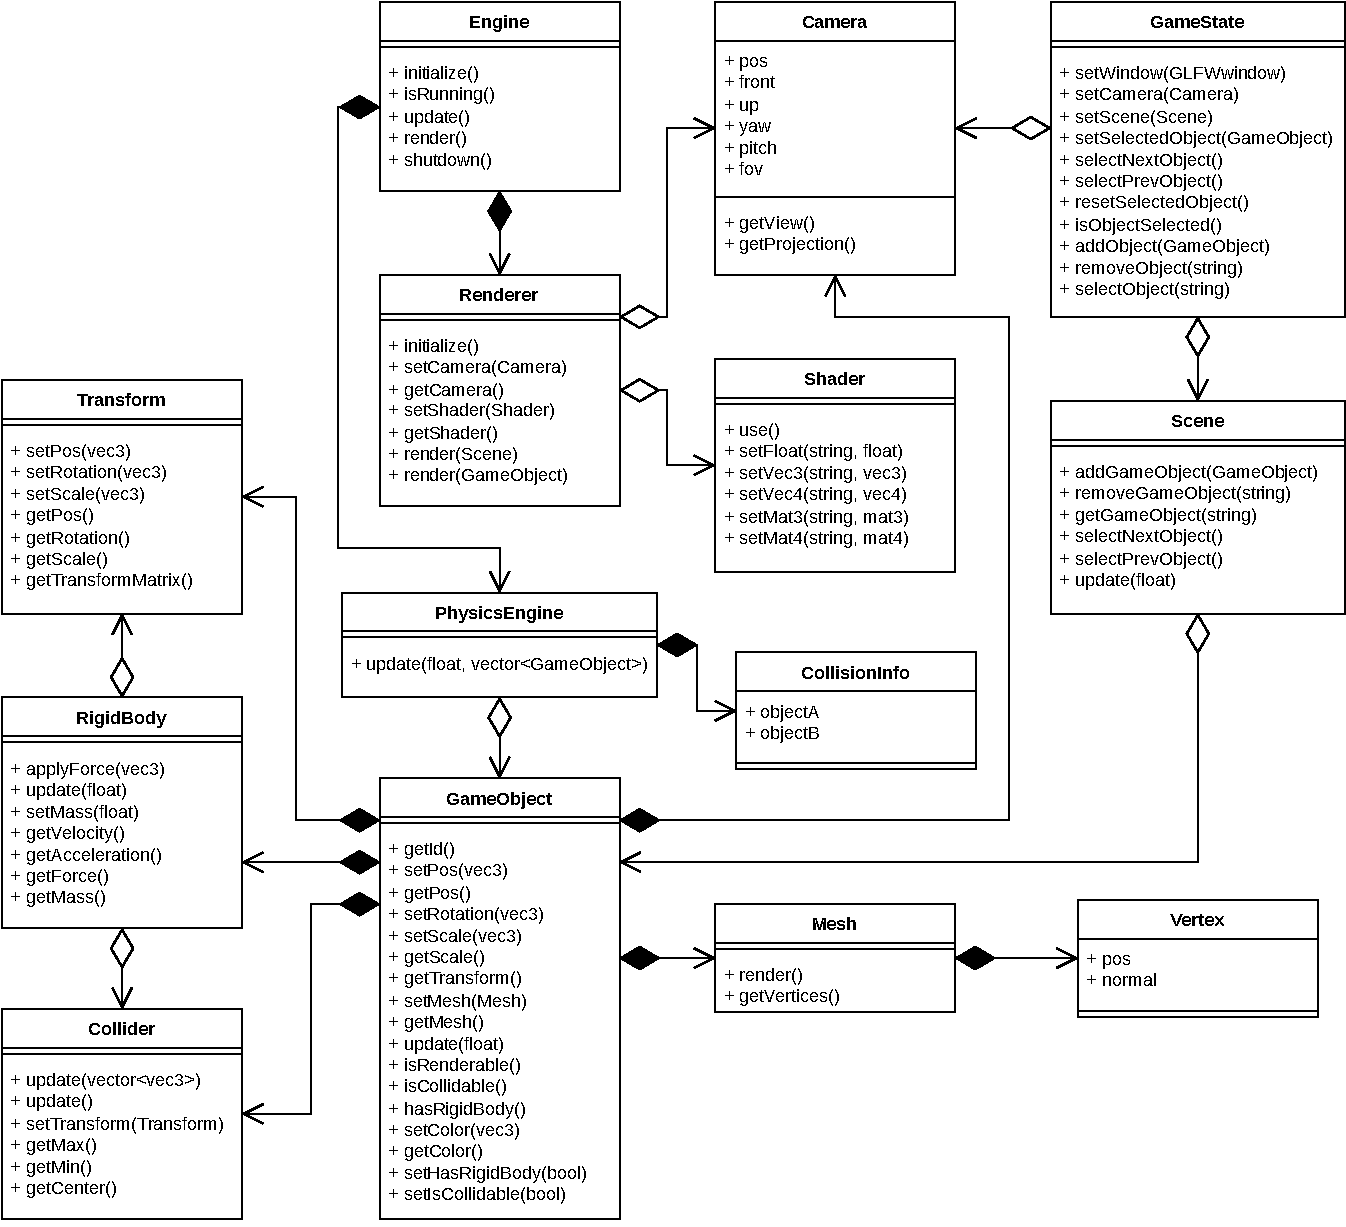
\includegraphics[width=\textwidth]{diag/uml.pdf}
	\caption{Диаграмма классов разработанного ПО}
	\label{fig:uml}
\end{figure}

\subsubsection*{Engine}

Класс Engine является центральным компонентом разработанного ПО, он отвечает за создание всех объектов, нужных для запуска приложения.
В главном цикле программы (см. Листинг \ref{lst:main}) он перенаправляет запросы на обработку ввода, обновление объектов и рендеринг сцены своим компонентам (PhysicsEngine и Renderer).

\begin{code}
    \begin{lstinputlisting}[
            label={lst:main},
            caption={Точка входа и главный цикл},
        ]{lst/main.cpp}
    \end{lstinputlisting}
\end{code}

\subsubsection*{PhysicsEngine}

Класс PhysicsEngine отвечает за обновление местоположения объектов в соответствии с атрибутами их компонента RigidBody (скорость, ускорение, сила и т.д.), обновление этих атрибутов на основе времени, прошедшего с момента генерации последнего кадра, а также обнаружение и разрешение коллизий между объектами.
Для обнаружения коллизий используются компоненты Collider объектов.
В случае обнаружения коллизий создаётся объект CollisionInfo, который хранит указатели на столкнувшиеся объекты.
Процесс обнаружения коллизий выглядит следующим образом:
\begin{enumerate}
    \item Для каждого объекта сцены, если он имеет компонент Collidable, добавить его во временный массив Collidables объектов, которые могут сталкиваться.
    \item Для каждой пары объектов из массива Collidables проверить, сталкиваются они или нет.
    \item Если объекты сталкиваются, создать объект CollisionInfo и добавить его во временный массив пар сталкивающихся объектов Collisions.
    \item Для каждой пары объектов из массива Collisions разрешить коллизии, обновив местоположения объектов и их физические характеристики.
\end{enumerate}

\subsubsection*{Renderer}

Класс Renderer отвечает за рендеринг объектов сцены и генерацию кадра.
Рендеринг происходит следующим образом:
\begin{enumerate}
    \item Для каждого объекта сцены, вызывается функция render класса Renderer.
    \item В функции render класса Renderer используются компоненты Mesh, Color и Transform объекта сцены: переменные шейдера инициализируются соответствующими данными компонентов Color и Transform, после чего вызывается функция render компонента Mesh.
    \item В функции render компонента Mesh происходит вызов функций OpenGL, в результате чего происходит отрисовка объекта.
\end{enumerate}

\subsubsection*{GameState}

Класс GameState, реализующий паттерн Одиночка, предназначен для хранения глобального состояния программы.
Получение указателей на текущую камеру, сцену и выбранный объект происходит по запросу к GameState.
Часть интерфейса класса GameState представлена на листинге \ref{lst:GameState}.

\begin{code}
    \begin{lstinputlisting}[
            label={lst:GameState},
            caption={Класс GameState},
        ]{lst/GameState.h}
    \end{lstinputlisting}
\end{code}

\subsection{Интерфейс}

На рисунках ниже представлен интерфейс программы.

\begin{figure}[H]
	\centering
	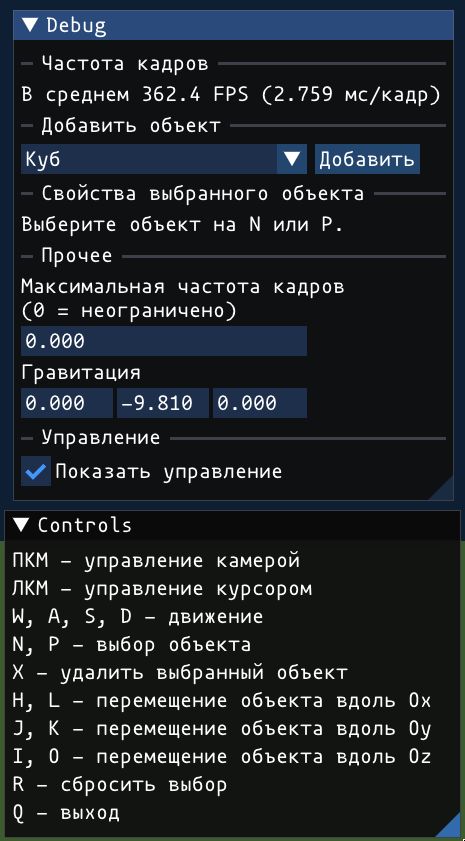
\includegraphics[width=0.6\textwidth]{img/demo-icontrols.png}
	\caption{Демонстрация интерфейса, объект не выбран}
	\label{fig:controls}
\end{figure}

\begin{figure}[H]
	\centering
	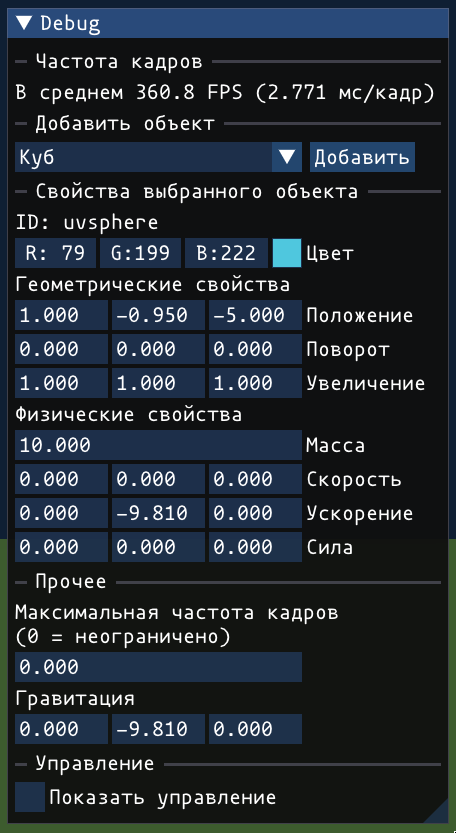
\includegraphics[width=0.6\textwidth]{img/demo-iobject.png}
	\caption{Демонстрация интерфейса, объект выбран}
	\label{fig:object}
\end{figure}

\subsection{Демонстрация работы программы}

На рисунках ниже представлена демонстрация работы программы.

\begin{figure}[H]
	\centering
	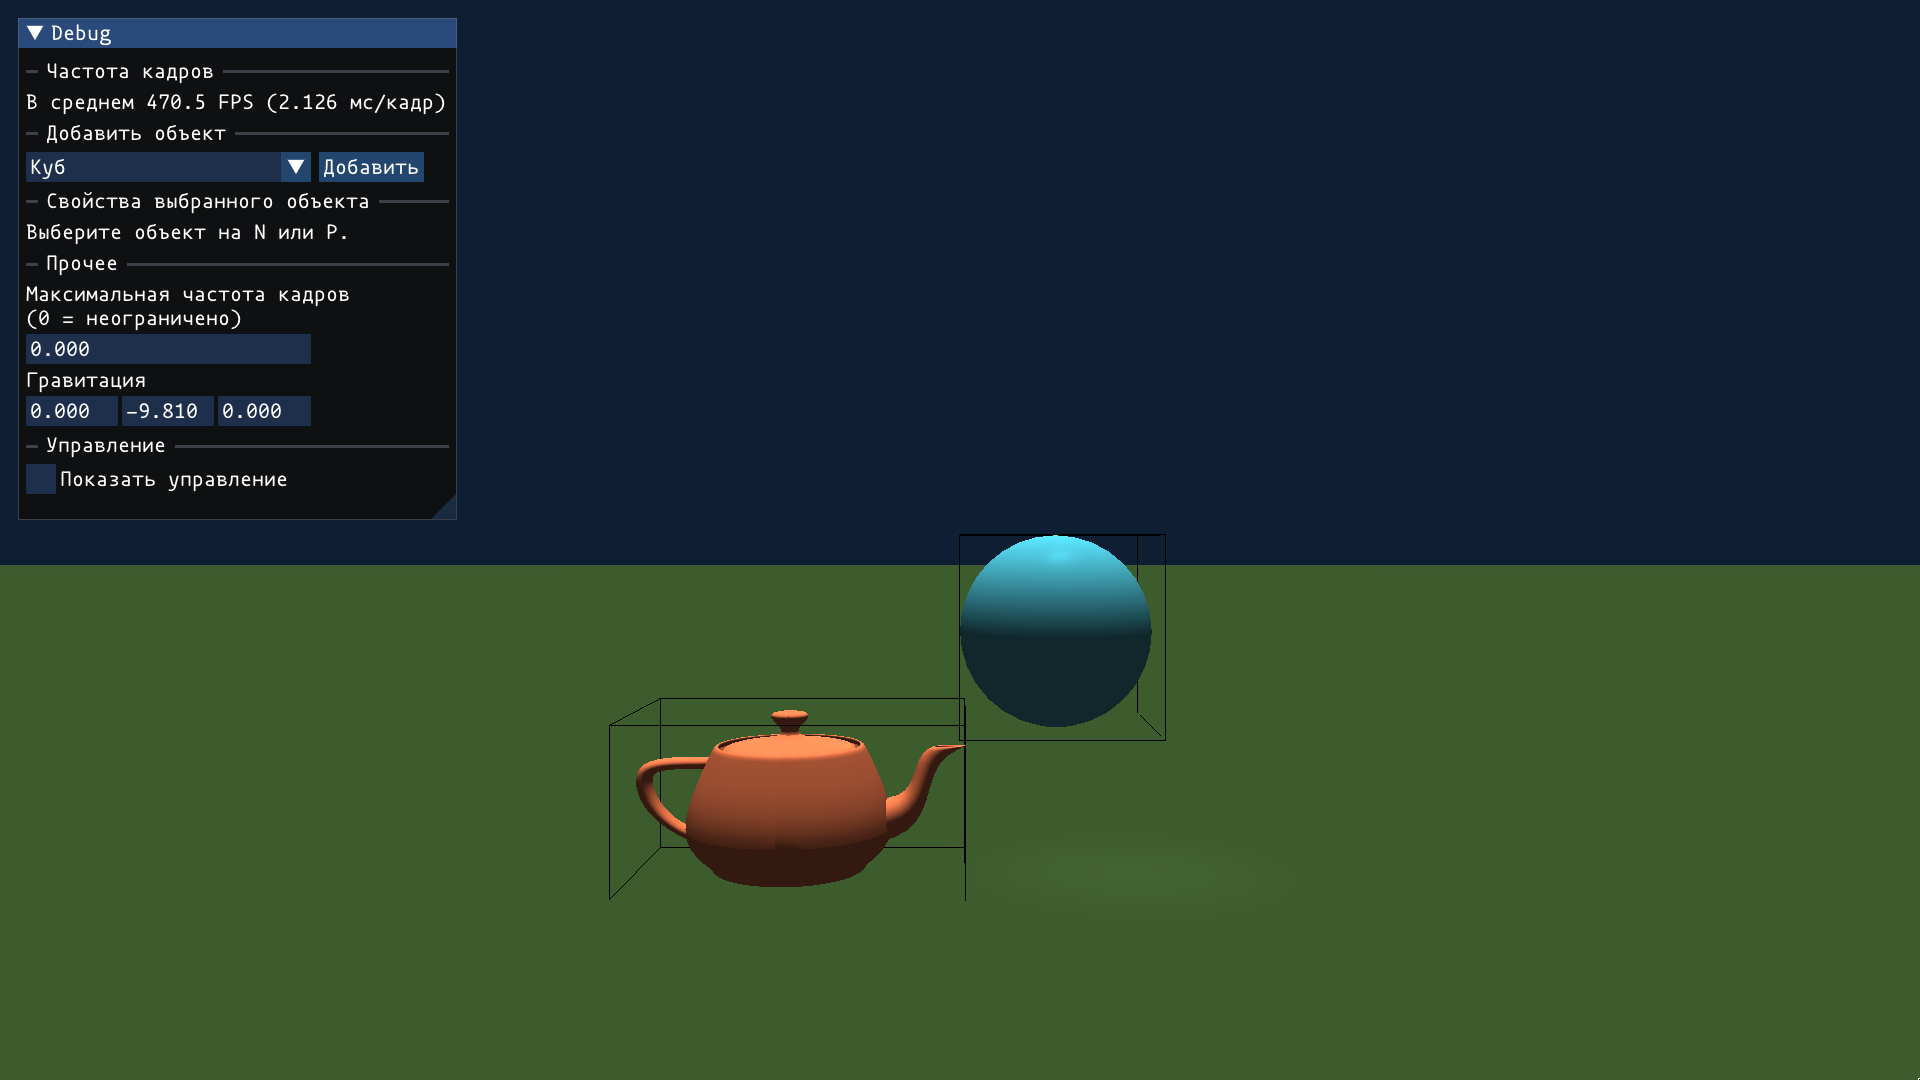
\includegraphics[width=\textwidth]{img/demo-start.png}
	\caption{Демонстрация работы программы сразу после запуска}
	\label{fig:start}
\end{figure}

\begin{figure}[H]
	\centering
	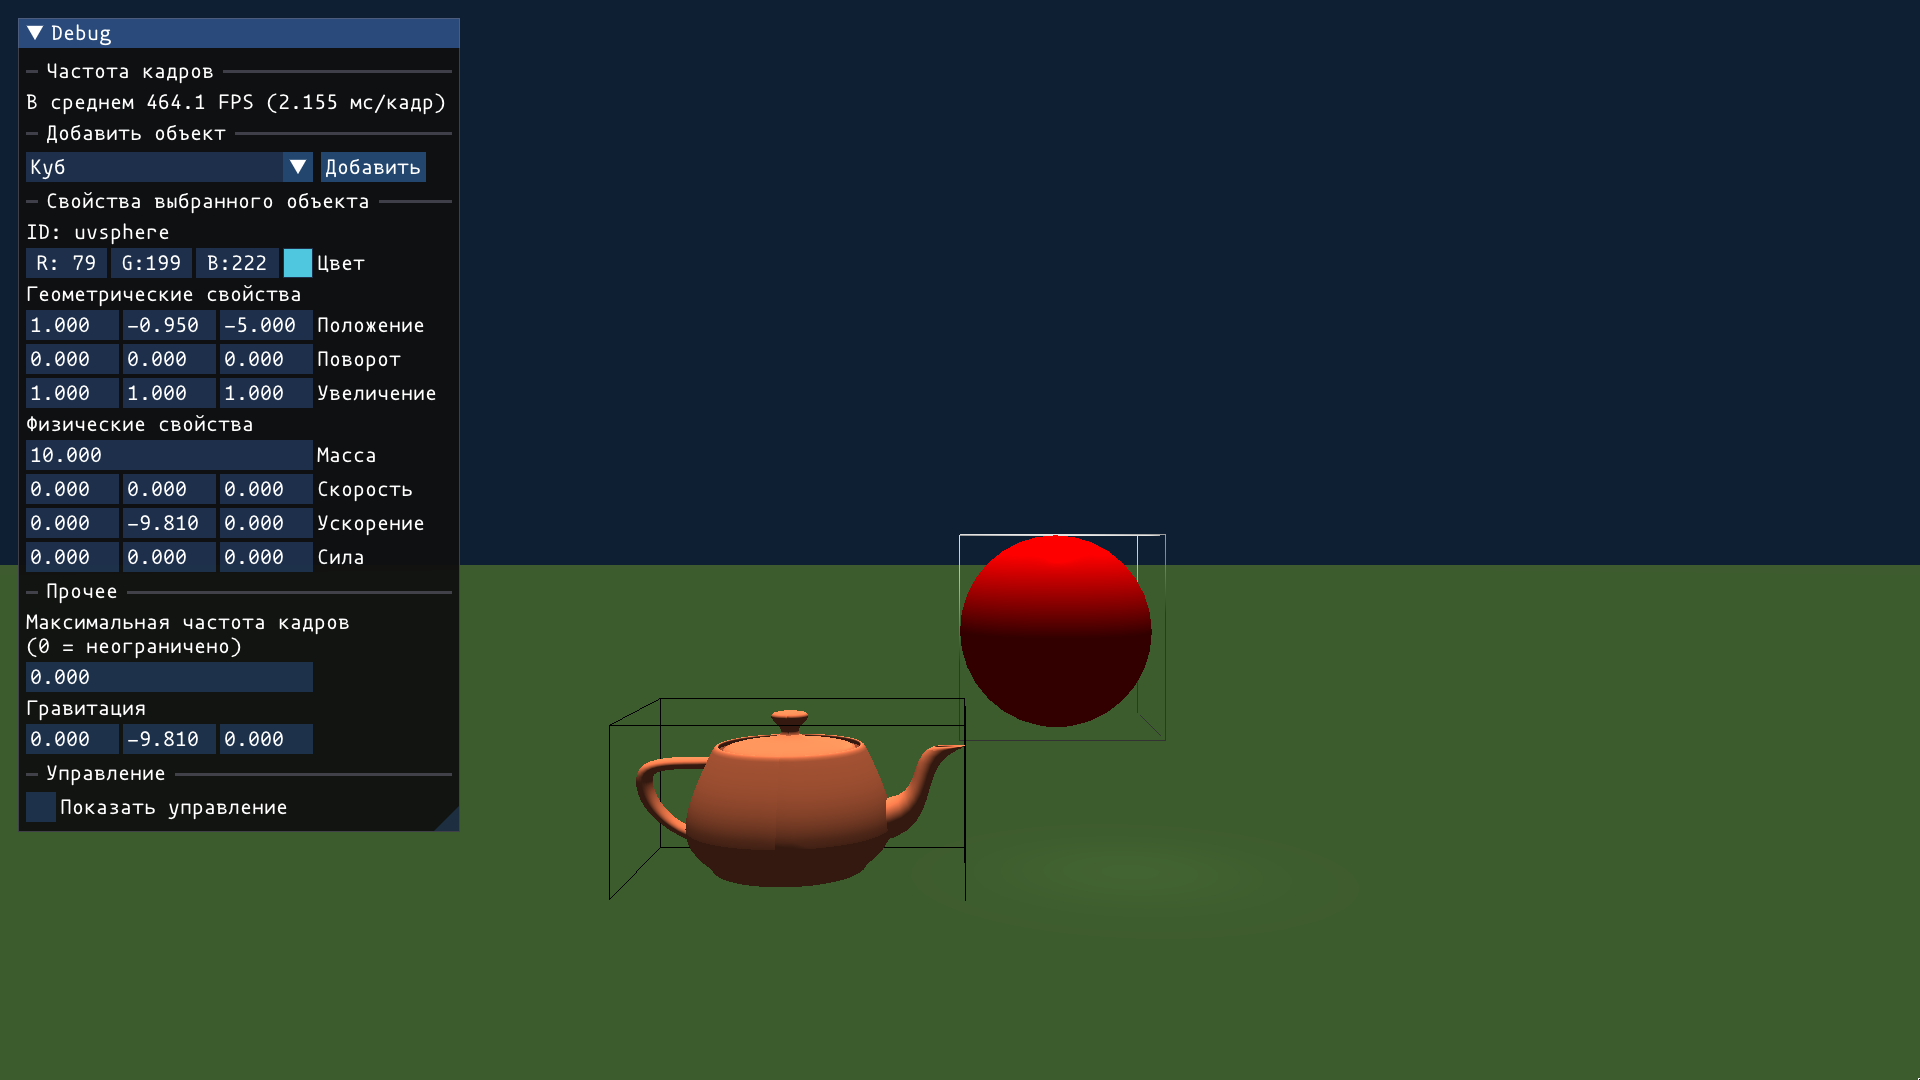
\includegraphics[width=\textwidth]{img/demo-select.png}
	\caption{Демонстрация выбора объекта}
	\label{fig:select}
\end{figure}

\begin{figure}[H]
	\centering
	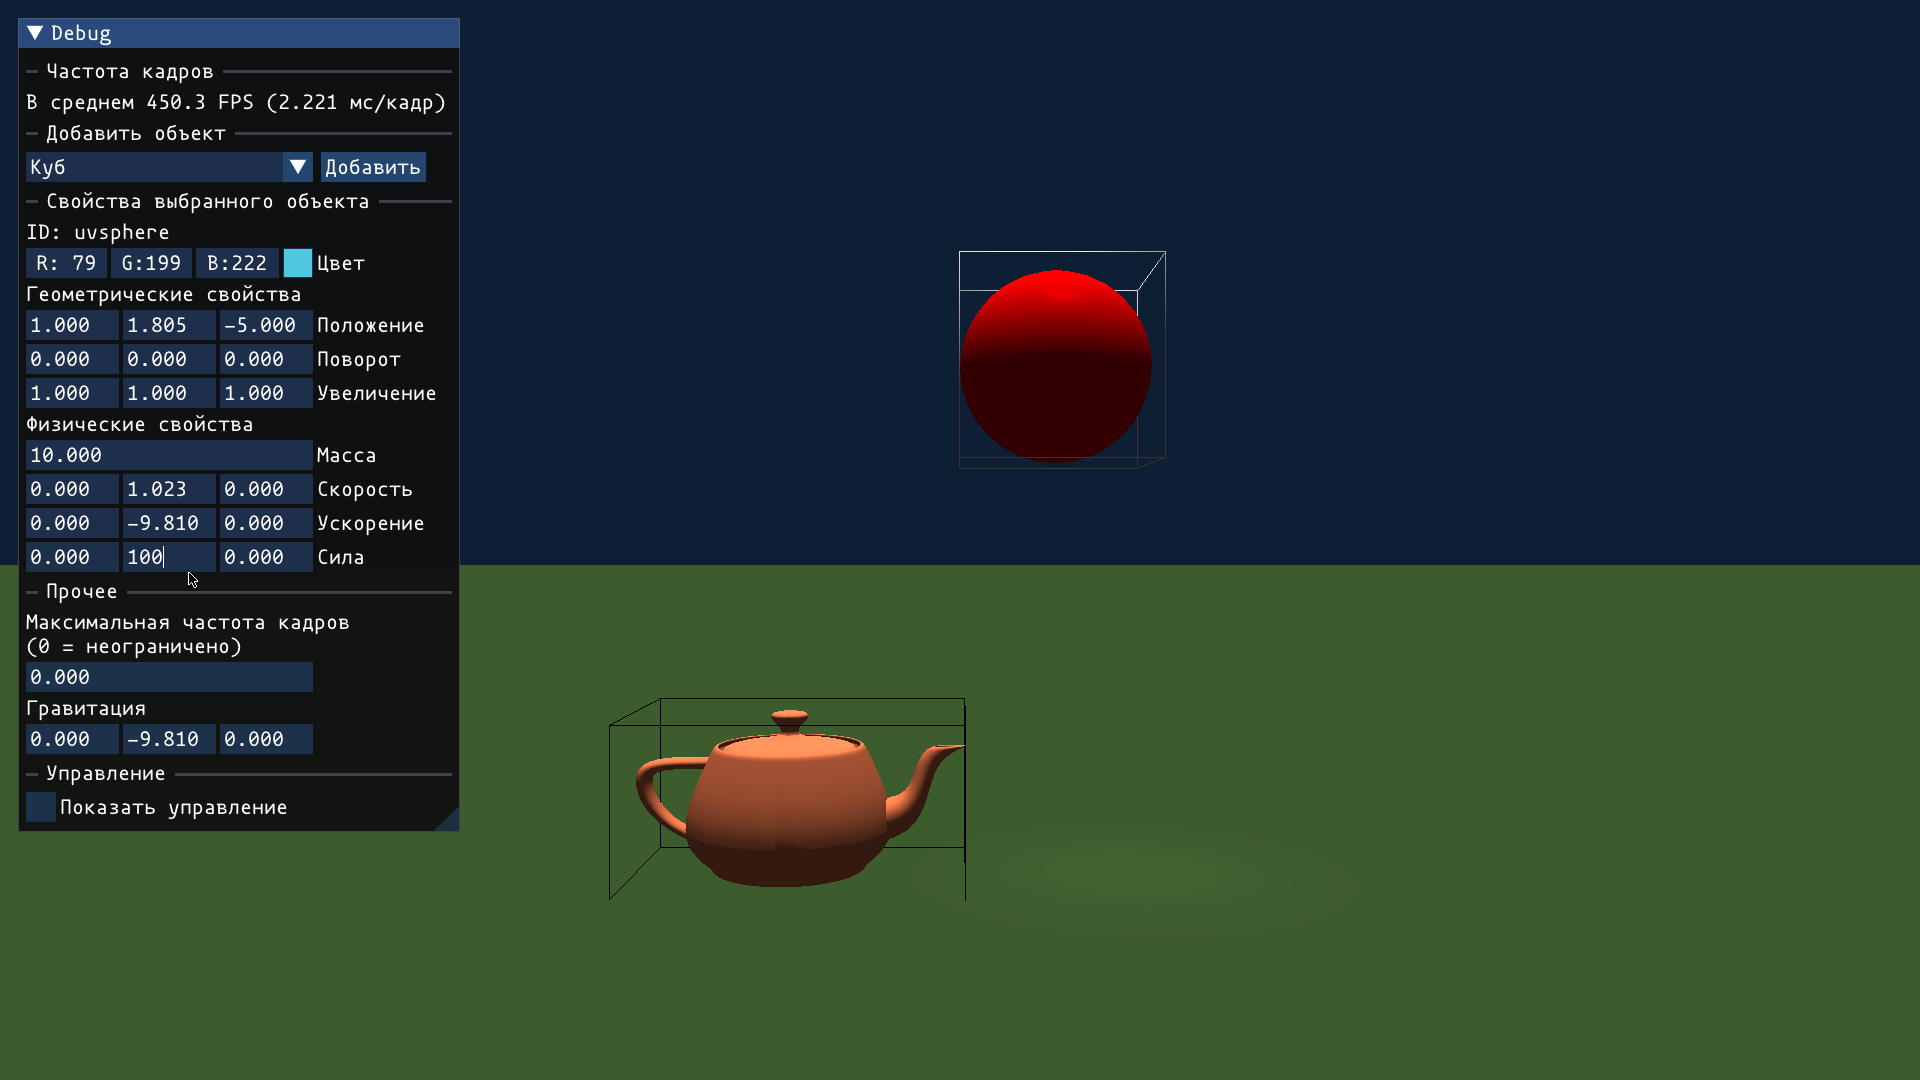
\includegraphics[width=\textwidth]{img/demo-force.png}
	\caption{Демонстрация приложения силы к объекту}
	\label{fig:force}
\end{figure}

\begin{figure}[H]
	\centering
	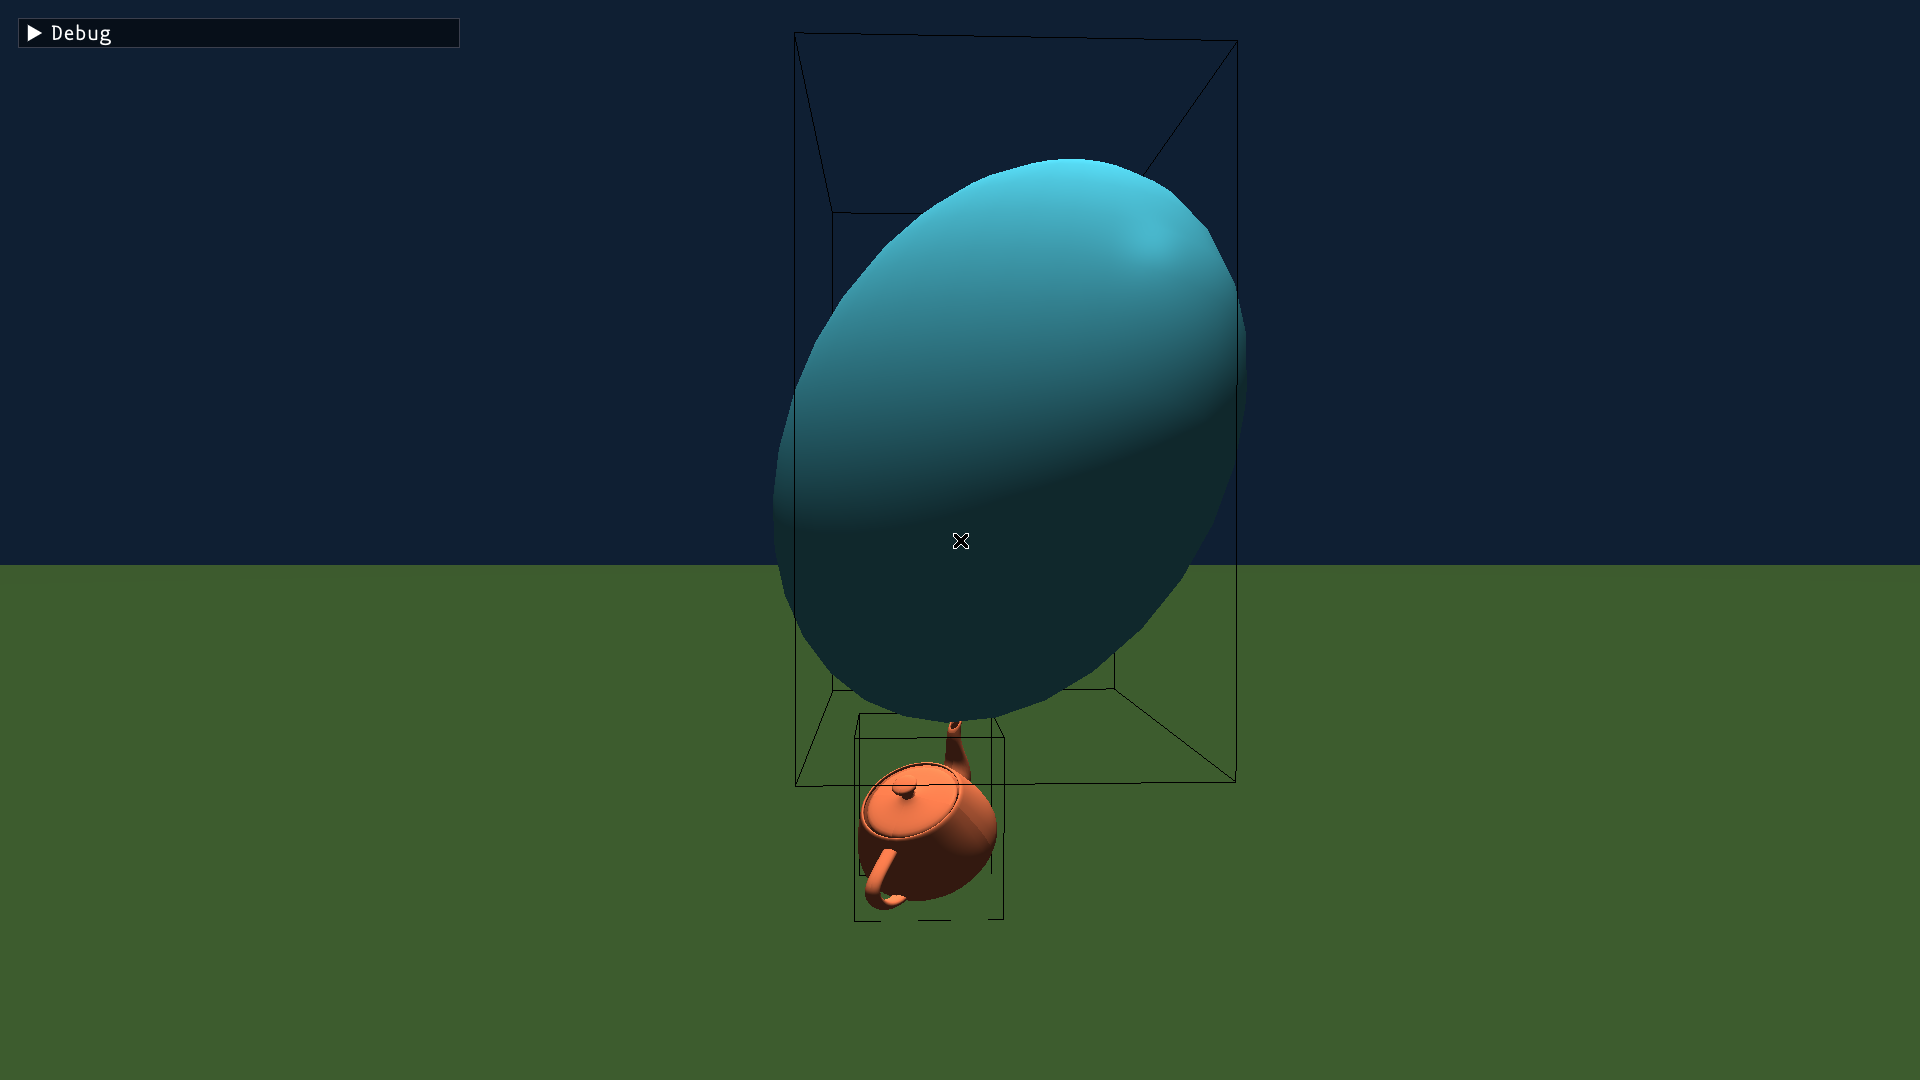
\includegraphics[width=\textwidth]{img/demo-transform.png}
	\caption{Демонстрация перемещения, поворота и масштабироавния объектов}
	\label{fig:transform}
\end{figure}

\begin{figure}[H]
	\centering
	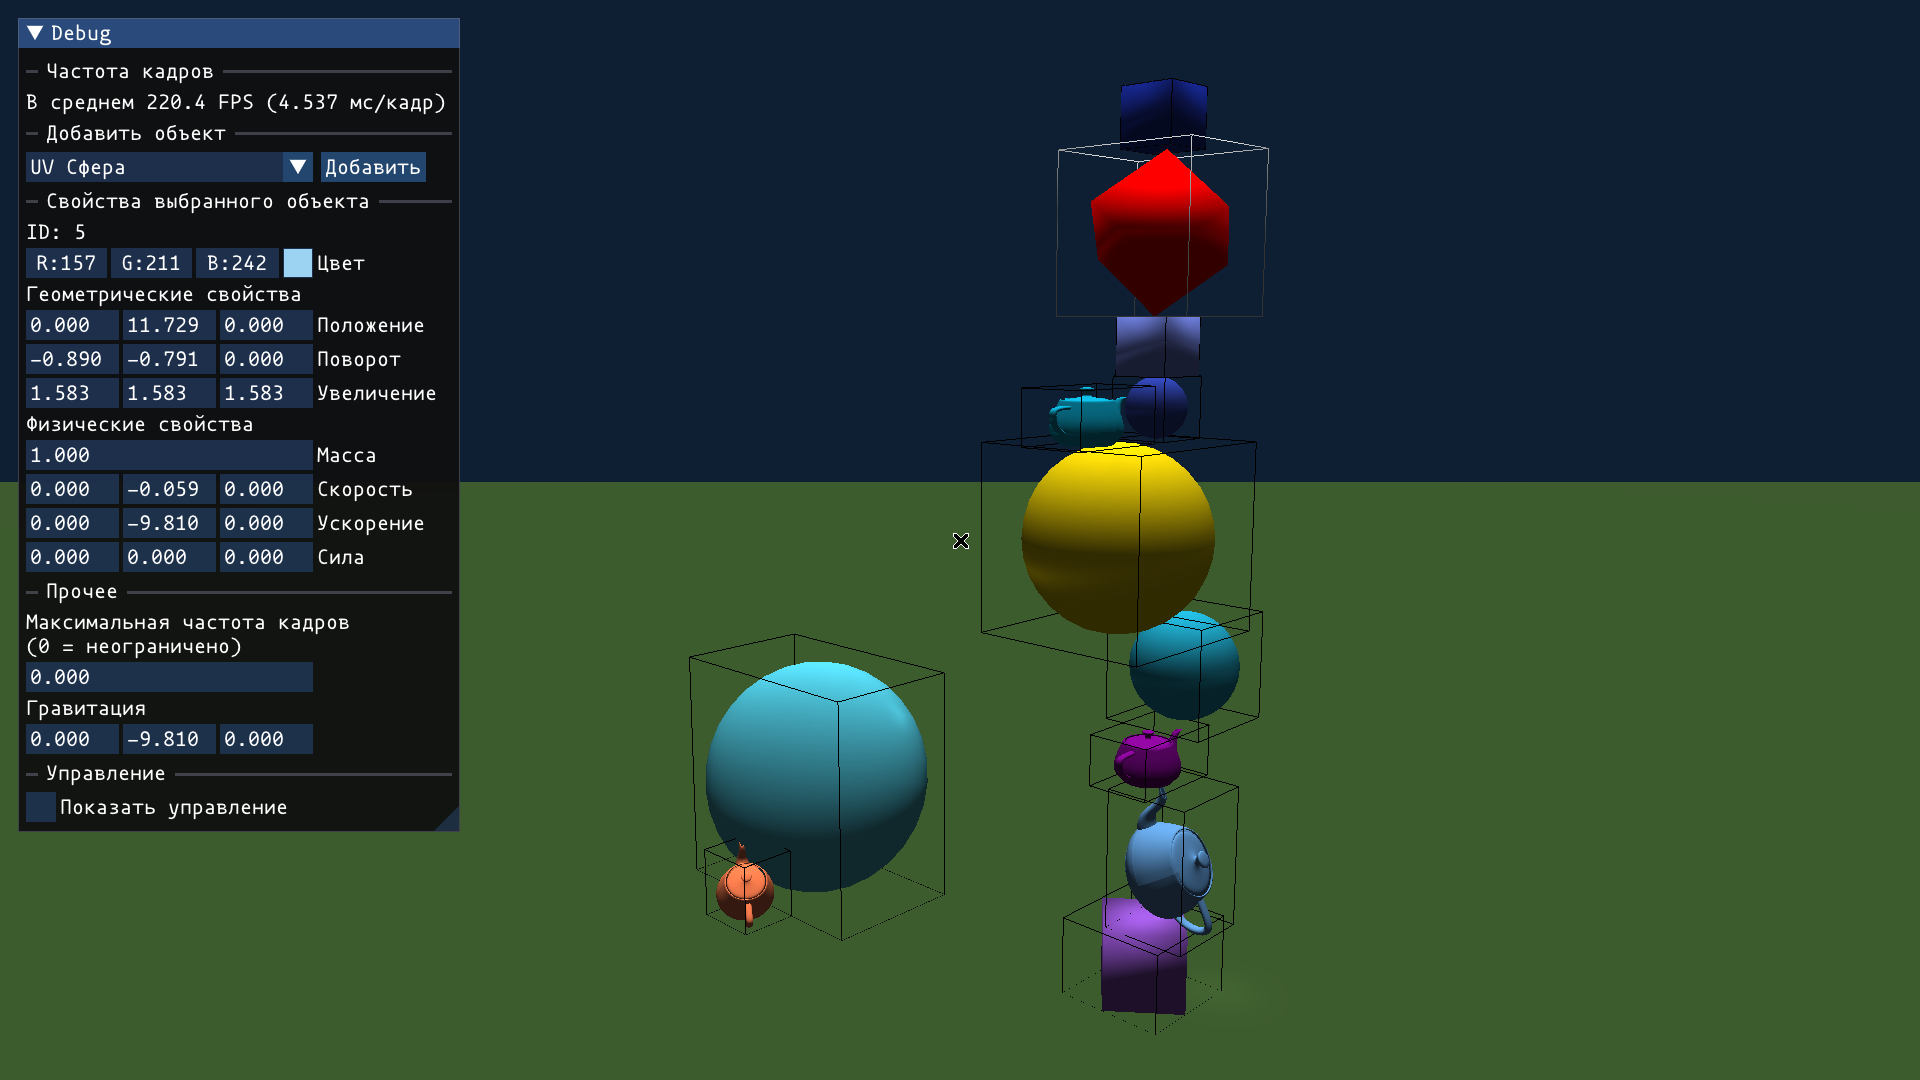
\includegraphics[width=\textwidth]{img/demo-spawn.png}
	\caption{Демонстрация создания объектов}
	\label{fig:spawn}
\end{figure}

\begin{figure}[H]
	\centering
	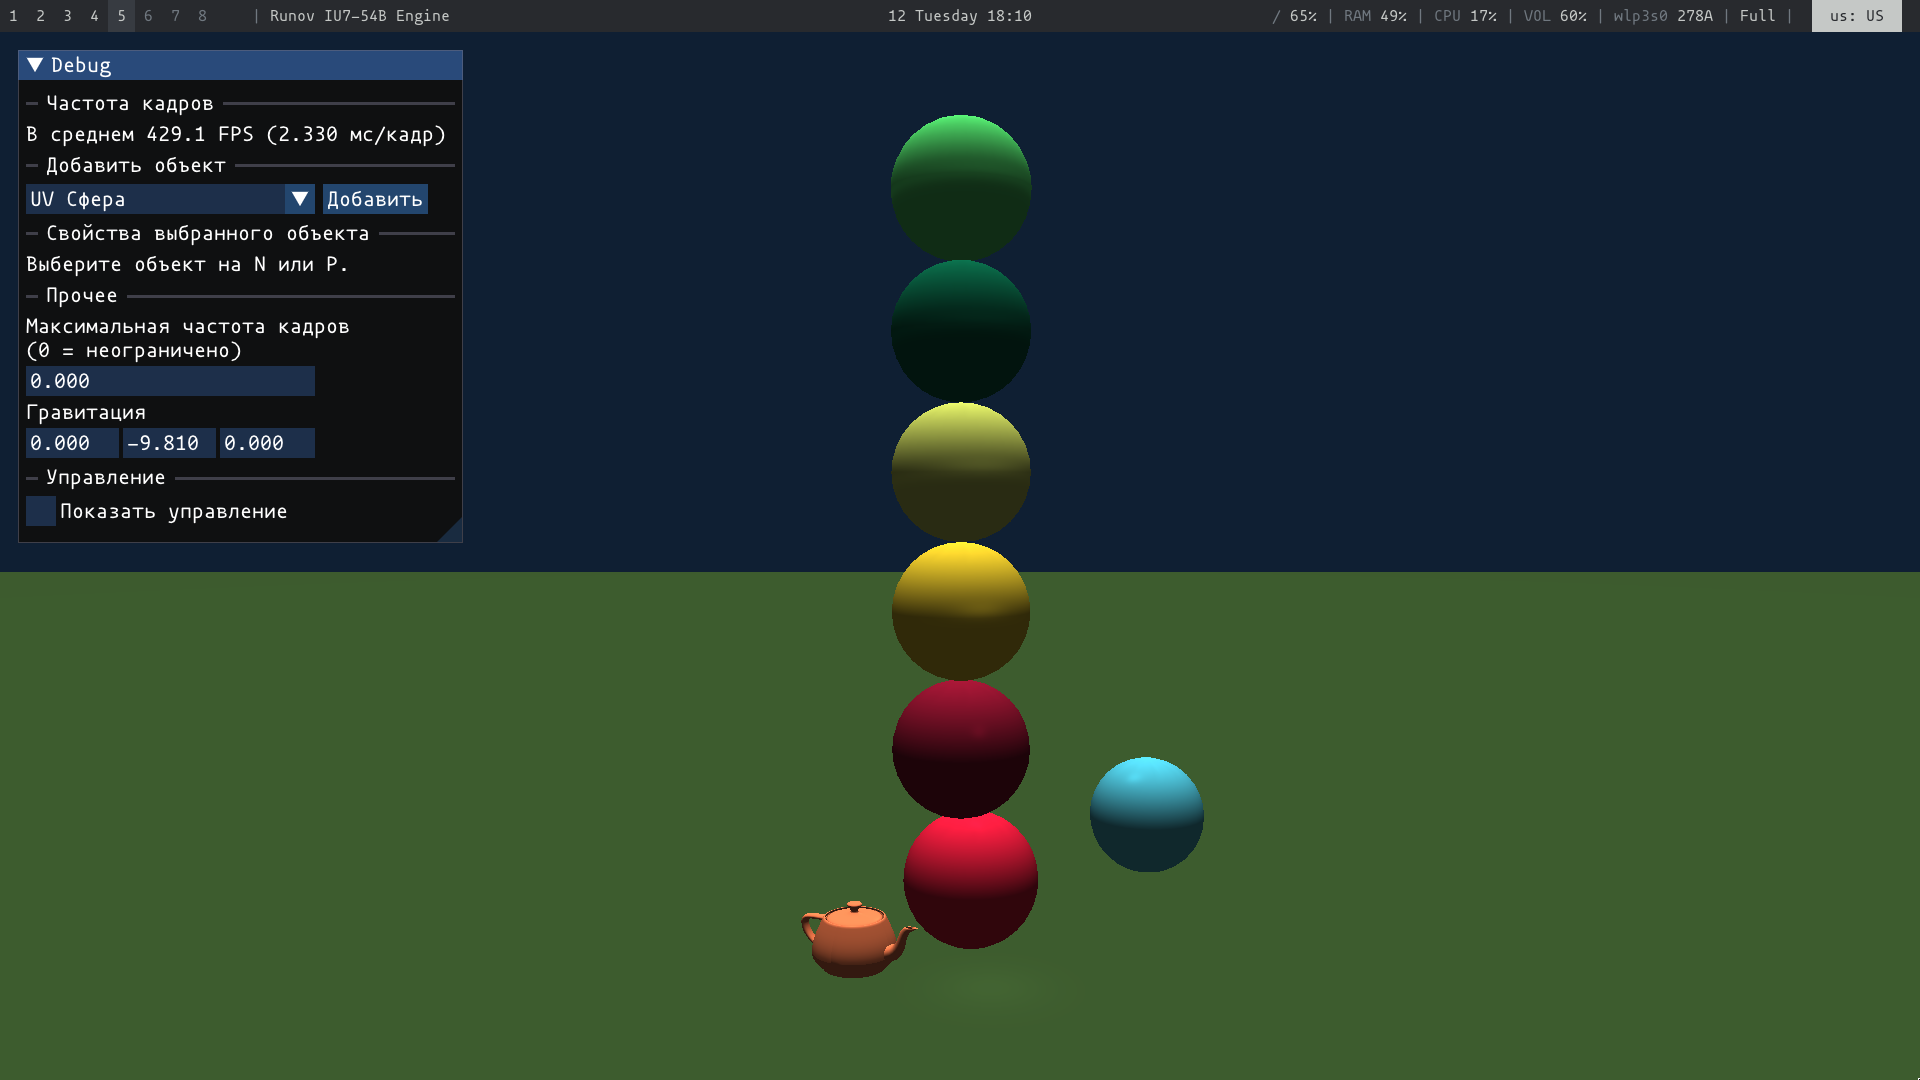
\includegraphics[width=\textwidth]{img/demo-nodbg.png}
	\caption{Демонстрация отключения визуализации AABB-коллайдеров объектов}
	\label{fig:nodbg}
\end{figure}

\newpage
\subsection{Вывод}

В данной части был обоснован выбор графического API, языка программирования и среды разработки, которые были использованы при разработке программного обеспечения.
Также была приведена UML-диаграмма классов, описывающая структуру программы.
Был продемонстрирован интерфейс, и приведены примеры работы программы.
